
\section{Special Perturbations}
The oblateness perturbation is one of the principal perturbing accelerations acting on Earth satellites from LEO to GEO, although its strength decays relatively rapidly with the orbital radius. Departures of the gravitational field from the spherical symmetry due to finer variations in the Earth's mass distribution are captured through a perturbing potential. Perturbations due to small longitudinal asymmetries (i.e., along the parallels) are particularly important for geostationary orbit, as they affect the stability of satellites on the geostationary ring. This section we look into the derivation and theory behind the gravitational potential function, how to interpret it and arrive to the acceleration term that are use in propagations. 
\vspace{0.3cm}
\hrule\vspace{0.1cm}
\hrule
\vspace{0.3cm}
\begin{multicols}{2}
\subsection{Gravitational Potential Model}
Given that the gradient of the potential for a spherical central body will yield the acceleration, we must examine how to form a \textbf{potential function} that includes the perturbing accelerations due to nonspherical central body.\par

\subsubsection{Deriving the Aspherical-Potential Function}
If we examine an infinite number of masses, $m_Q$, at point $Q$, the potential oer unit mass at point $P$ is the summation of the potential due to each of these points, and the acceleration is $\nabla U$. Suppose $\rho$ is the radius from the point mass $m_Q$ to the spacecraft. The change in potential sue to an infinitesimal element of mass, $dm_\oplus$, is
\begin{gather}
    U = G\sum_{Q=1}^{\infty}\frac{m_Q}{\rho_Q},\hspace*{1cm}dU = g\frac{dm_\oplus}{\rho_Q}
\end{gather}
Considering Earth as being composed by a set of such infinitesimal masses (see \hyperref[fig:point_mass]{Fig. (\ref*{fig:point_mass})}), each giving a contribution of $dU$ to the total Gravitational potential, thus, the summation of each mass approaches an integral and can be express as
\begin{gather}
    U = G\underset{body}{\int}\frac{1}{\rho_Q}dm_\oplus
    \label{eq:int_mass}
\end{gather}
To relate the potential to the position vector of the spacecraft with respect to the Earth's centre of mass $\mathbf{r}$, we can express $\rho$ using the law of cosines,
\begin{gather}
    \mathbf{\rho_Q} = \mathbf{r} - \mathbf{r_Q} = \sqrt{r^2+r_Q^2-2rr_Q\COS(\Lambda)}
\end{gather}
where the angle $\COS(\Lambda)$ can be determined using dot product, $\COS(\Lambda)=(\mathbf{r}\cdot\mathbf{r_Q}/(rr_Q))$. Substitute the above equation into \hyperref[eq:int_mass]{Eq. (\ref*{eq:int_mass})}, the potential of the body then becomes
\begin{gather}
    \begin{split}
        U &= \underset{body}{\int}\frac{dm_\oplus}{\sqrt{r^2+r_Q^2-2rr_Q\COS(\Lambda)}}\\
          &= \underset{body}{\int}\frac{dm_\oplus}{r\sqrt{1+\alpha^2-2\alpha\COS(\Lambda)}}
    \end{split}
\end{gather}
Where $\alpha = r_Q/r$. The parameter ($\alpha$) will always be $\alpha<1$ because the spacecraft (point) is outside of the central body ($r>R_\oplus$). Thus, we can use the binomial theorem to expand the denominator of the potential in a series.
\begin{gather}
    \begin{split}
        \frac{1}{\sqrt{1-2\alpha\COS(\Lambda)+\alpha^2}} = \frac{1}{\sqrt{1+x}} = \sum_{l=0}\alpha^lP_l[\COS(\Lambda)]
    \end{split}
\end{gather}
This expression is a series of \textit{Legendre polynomials}\footnote{The Legendre polynomials here is defined as the coefficients in a formal expression in powers of $\alpha$ of the \textit{generating function}. Generating functions is a way of encoding an infinite sequence of numbers by treating them as the coefficients of a formal power series. }, $P_l$. Setting $\gamma = \COS(\Lambda)$ for convenience, Rodriguez's formula gives the \textit{conventional} Legendre polynomials,
\begin{gather}
    \begin{split}
        P_l[\gamma] &= \frac{1}{2^ll!}\frac{d^l(\gamma^2-1)^l}{d\gamma^l}\\
        P_l[\gamma] &= \frac{1}{2^l}\sum_{j=0}^{\frac{l}{2}}\frac{(-1)^j(2l-2j)!}{j!(l-j)!(l-2j)!}\gamma^{l-2j}
    \end{split}
\end{gather}
The first six Legendre polynomials are,
\begin{gather}
    \begin{split}
        P_0[\gamma] &= 1\\
        P_1[\gamma] &= \gamma\\
        P_2[\gamma] &= \frac{1}{2}(3\gamma^2-1)\\
        P_3[\gamma] &= \frac{1}{2}(5\gamma^3-3\gamma)\\
        P_4[\gamma] &= \frac{1}{8}(35\gamma^4-30\gamma^2+3)\\
        P_5[\gamma] &= \frac{1}{8}(63\gamma^5-70\gamma^3+15\gamma)\\
        \label{eq:poly_terms}
    \end{split}
\end{gather}
Incorporating the concept of Legendre polynomials, we can write the potential as
\begin{gather}
    U = \frac{G}{r}\underset{body}{\int}\sum_{l=0}^{\frac{l}{2}}\alpha^lP_l[\COS(\Lambda)]dm_\oplus
    \label{eq:Potential}
\end{gather}
The following section provides a detailed look into the implication of the potential equation. By combining the \textit{MacCullagh's formula} and the \textit{addition theorem} of spherical harmonics, we can thus derive a more comprehensive potential function to determine our acceleration for numerical propagations. 
\end{multicols}
\begin{figure}[H]
    \centering
    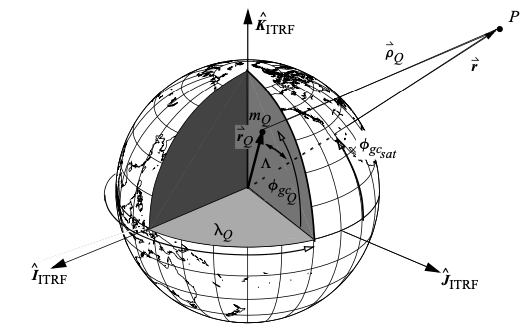
\includegraphics[width=.55\textwidth]{perturbation/point_mass.png}
    \caption{\textbf{Deriving the Gravitational Potential.} Schematic of Earth being composed with point masses, $m_Q$. Note that the frame is in ITRF\cite[]{}.}
    \label{fig:point_mass}
\end{figure}
\begin{multicols}{2}
\subsection{MacCullagh Geometric Method}
\subsubsection{MacCullagh's formula}
Using \textit{MacCullagh's} approach, we express the potential in \hyperref[eq:Potential]{Eq. (\ref*{eq:Potential})} as below. This permits us to evaluate each gravitational component and to exploit the implication of each gravitational potential term. 
\begin{gather}
    U = \underbrace{U_0}_\text{two body} + \underbrace{U_1}_\text{centre of mass}+ \underbrace{U_2}_\text{moments of inertia}+\dots
\end{gather}

\begin{enumerate}
    \item $\mathbf{U_0}$, \textit{\textbf{First Potential Term}}\\
    Using the first Legendre polynomial terms for the first term $P_0$, 
    \begin{gather}
        U_0 = \frac{G}{r}\int dm_{\oplus} = \frac{Gm_\oplus}{r}=\frac{\mu}{r}
    \end{gather}
    Conveniently, what the the first term, $U_0$, assumed is that the central body is spherically symmetric and homogeneous, which is what we often referred as the \textit{two-body} potential.
    \vspace*{0.3cm}
    \item $\mathbf{U_1}$, \textit{\textbf{Second Potential Term}}\\
    using the Legendre polynomial term by letting $l=1$ and the expression of $\COS(\Lambda)$ from dot product manipulation, 
    \begin{gather}
        \begin{split}
            U_1 &= \frac{G}{r}\int\COS(\Lambda)\alpha dm_\oplus = \frac{G}{r}\int\frac{x\xi+y\eta+z\zeta}{r^2}dm_\oplus\\[0.2cm]
                &= \frac{G}{r^3}\Big(x\int\xi dm_\oplus + y\int\eta dm_\oplus + z\int\zeta dm_\oplus\Big)
        \end{split}
    \end{gather}
    Each integral (for $\xi,\eta$, and $\zeta$) represents the component of the potential to account for a displacement of the centre of mass from the origin of the coordinate frame. Even if the origin coincides with the geometric centre of the body, it may not coincide with the centre of mass. However, if the origin coincides with the centre of mass, 
    \begin{gather}
        \int\xi dm_\oplus = \int\eta dm_\oplus = \int\zeta dm_\oplus = 0
    \end{gather}
    Thus, $U_1=0$ because the origin we chose is at the centre of mass. The expressions above are definitions of the centre of mass. 
    \vspace*{0.3cm}
    \item $\mathbf{U_2}$, \textit{\textbf{Third Potential Term}}\\
    The third term in the expansion is
    \begin{gather}
        U_2 = \frac{1}{2}\frac{G}{r^3}\int(3\gamma^2-1)r_Q^2dm_\oplus
    \end{gather}
    and since we defined $\gamma = \COS(\Lambda)$, we can substitute it in
    \begin{gather}
        U_2 = \frac{G}{2r^3}\underbrace{\int2r_Q^2dm_\oplus}_{A+B+C} - \frac{G}{2r^3}\underbrace{\int3r_Q^2\SIN^2(\Lambda)dm_\oplus}_{I}
    \end{gather}
    where $A,B$ and $C$ represents the \textit{moments of inertia} about the three coordinate axes 
    \begin{gather}
        \begin{split}
            A &= \int(\eta^2+\zeta^2)dm_\oplus\\
            B &= \int(\zeta^2+\xi^2)dm_\oplus\\
            C &= \int(\xi^2+\eta^2)dm_\oplus\\
        \end{split}
    \end{gather}
    And the remaining term is the \textit{polar moment of inertia}, $I$, that refers to any point $r_Q$
    \begin{gather}
        I = \int r_Q^2\SIN^2(\Lambda)dm_\oplus
    \end{gather}
    Thus, we can rewrite the second potential term as
    \begin{gather}
        U_2 = \frac{G}{2r^3}(A+B+C-3I)
    \end{gather}
\end{enumerate}

By substituting all the terms ($U_0$-$U_2$) and assuming the coordinate frame's origin is at the centre of mass, gives us the aspherical potential 
\begin{gather}
    U = \frac{Gm_\oplus}{r}+\frac{G}{2r^3}(A+B+C-3I)
\end{gather}
This is the \textit{MacCullagh's formula}. Note that evaluating the integrals defining $A,B,C$ and $I$ presents practical problem requiring detailed knowledge on Earth's mass distribution, which is often quite unrealistic to assume uniform density. Therefore, we need to incorporate an alternative by introducing a geometric approach for \hyperref[eq:Potential]{Eq. (\ref*{eq:Potential})}.

\subsubsection{Geometric Approach (Spherical Harmonics)}
The \textit{geometric approach} examines the potential function and incorporate spherical trigonometry to develop an equation to find the angle, $\Lambda$, directly. Noe that a satellite's latitude will always be a $geocentric$ value ($\phi_{gc_{sat}}$). If we substitute $\phi_{gc_{sat}}$ with $\Lambda$, and using cosine law of spherical trigonometry,
\begin{gather}
    \begin{split}
    \COS(\Lambda) &= \COS(90^\circ - \phi_{gc_{Q}})\COS(90^\circ - \phi_{gc_{sat}})\\
                  &+\SIN(90^\circ - \phi_{gc_{Q}})\SIN(90^\circ - \phi_{gc_{sat}})\COS(\lambda_Q-\lambda_{sat})
    \end{split}
\end{gather}
Reduction gives us
\begin{gather}
    \begin{split}
        \COS(\Lambda)&=\SIN(\phi_{gc_{Q}})\SIN(\phi_{gc_{sat}})\\
        &+\COS(\phi_{gc_{Q}})\COS(\phi_{gc_{sat}})\COS(\lambda_Q-\lambda_{sat})
    \end{split}
\end{gather}
The \textit{addition theorem} of spherical harmonics provides a way to expand the expression for $\Lambda$ into \hyperref[eq:Potential]{Eq. (\ref*{eq:Potential})}

\begin{gather}
    \begin{split}
        P_l[\COS(\Lambda)] &= P_l[\SIN(\phi_{gc_{Q}})]P_l[\SIN(\phi_{gc_{sat}})]\\
                    &+2\sum_{m=1}^{l}\frac{(l-m)!}{(l+m)!}\{A_{l,m}A'_{l,m}+B_{l,m}B'_{l,m}\}
    \end{split}
\end{gather}
\begin{gather*}
    \begin{split}
        A_{l,m} &= P_{l,m}[\SIN(\phi_{gc_{Q}})]\COS(m\lambda_Q)\\
        A'_{l,m} &= P_{l,m}[\SIN(\phi_{gc_{sat}})]\COS(m\lambda_{sat})\\
        B_{l,m} &= P_{l,m}[\SIN(\phi_{gc_{Q}})]\SIN(m\lambda_Q)\\
        B'_{l,m} &= P_{l,m}[\SIN(\phi_{gc_{sat}})]\SIN(m\lambda_{sat})\\
    \end{split}
\end{gather*}
where the summation introduces "$l$" and "$m$" indices as \textit{degree} and \textit{order}, respectively. The term $P_{l,m}$ are called the \textit{associated} Legendre functions, $P_{l,m}$. Notice that for zero order ($m=0$), the associated Legendre functions are simply the conventional Legendre polynomials. The general form were given by Lambeek as the following
\begin{gather*}
    P_{l,m}[\gamma] = \frac{1}{2^ll!}(1-\gamma^2)^{m/2}\frac{d^{l+m}}{d\gamma^{l+m}}(\gamma^2-1)^l
\end{gather*}

\begin{center}
    \begin{tabular}{ccc}
        $l$ & $m$ & $P_{l,m}(\SIN\phi)$ \\[0.1cm]
        \hline\hline
        0   & 0   & 1 \\[0.1cm]
        \hline
        1   & 0   & $\SIN(\phi_{gc_{sat}})$ \\[0.1cm]
        1   & 1   & $\COS(\phi_{gc_{sat}})$ \\[0.1cm]
        \hline
        2   & 0   & $\frac{1}{2}\{3\SIN^2(\phi_{gc_{sat}})-1\}$ \\[0.1cm]
        2   & 1   & $3\SIN(\phi_{gc_{sat}})\COS(\phi_{gc_{sat}})$ \\[0.1cm]
        2   & 2   & $3\COS^2(\phi_{gc_{sat}})$ \\[0.1cm]
        \hline
        3   & 0   & $\frac{1}{2}\{5\SIN^3(\phi_{gc_{sat}})-3\SIN(\phi_{gc_{sat}})\}$ \\[0.1cm]
        3   & 1   & $\frac{1}{2}\COS(\phi_{gc_{sat}})\{15\SIN^2(\phi_{gc_{sat}})-3\}$ \\[0.1cm]
        3   & 2   & $15\COS^2(\phi_{gc_{sat}})\SIN(\phi_{gc_{sat}})$ \\[0.1cm]
        3   & 3   & $15\COS^3(\phi_{gc_{sat}})$ \\[0.1cm]
        \hline\hline
    \end{tabular}
\end{center}


By separating all the terms that are independent of the satellite's location in \hyperref[eq:Potential]{Eq. (\ref*{eq:Potential})}, we can arrive at a solution that isolates terms which depends only on the central body and those which relate that satellite's position. FIrst we define two new variables, $C'_{l,m}$ and $S'_{l,m}$, as follow
\begin{gather}
    \begin{split}
        C'_{l,m} &= \underset{body}{\int}r_Q^l\frac{(l-m)!}{(l+m)!}P_{l,m}[\SIN(\phi_{gc_{sat}})]\COS(m\lambda_Q)dm_\oplus\\
        S'_{l,m} &= \underset{body}{\int}r_Q^l\frac{(l-m)!}{(l+m)!}P_{l,m}[\SIN(\phi_{gc_{sat}})]\SIN(m\lambda_Q)dm_\oplus
    \end{split}
\end{gather}
The two coefficients, $C'_{l,m}$ and $S'_{l,m}$, represent the mathematical modelling for the Earth's shape using spherical harmonics. The special case for the \textit{zonal harmonics} is 
\begin{gather}
    C'_{l,0}=\underset{body}{\int}r_Q^lP_l[\SIN(\phi_{gc_{Q}})]dm_\oplus
\end{gather}
which uses the conventional Legendre polynomials. Note that $S'_{l,0}$ is zero. Substitute these values into the potential in \hyperref[eq:Potential]{Eq. (\ref*{eq:Potential})} we can get the following expression for our potential. 
\end{multicols}
\par\noindent\rule{\dimexpr(0.5\textwidth-0.5\columnsep-0.4pt)}{0.4pt}%
\rule{0.4pt}{6pt}

\begin{gather}
    \begin{split}
        U &= \frac{G}{r}\sum_{l=0}^{\infty}\frac{P_l[\SIN(\phi_{gc_{sat}})]}{r^l}C'_{l,0}+\frac{G}{r}\sum_{l=1}^{\infty}\sum_{m=1}^{l}\frac{P_{l,m}[\SIN(\phi_{gc_{sat}})]}{r^l}\Bigg\{ C'_{l,m}\COS(m\lambda_{sat})+S'_{l,m}\SIN(m\lambda_{sat})\Bigg\}\\
        &= \frac{\mu}{r}\sum_{l=0}^{\infty}P_l[\SIN(\phi_{gc_{sat}})]\Big(\frac{R_\oplus}{r}\Big)^lC_{l,0} + \frac{\mu}{r}\sum_{l=1}^{\infty}\sum_{m=1}^{l}P_{l,m}[\SIN(\phi_{gc_{sat}})]\Big(\frac{R_\oplus}{r}\Big)^l\Bigg\{C_{l,m}\COS(m\lambda_{sat})+S_{l,m}\SIN(m\lambda_{sat})\Bigg\}
    \end{split}
\end{gather}

\vspace{\belowdisplayskip}\hspace{9.2cm}
\rule[-6pt]{0.4pt}{6.4pt}%
\rule{\dimexpr(0.5\textwidth-0.5\columnsep-0.4pt)}{0.4pt}%
\begin{multicols}{2}
A unit analysis suggest removing units from the above result. This leads to the $C$ and $S$ coefficients. We can undimensionalise the gravitational coefficients.
\begin{gather}
    C'_{l,m} = C_{l,m}R^l_\oplus m_\oplus,\hspace*{0.4cm}S'_{l,m} = S_{l,m}R^l_\oplus m_\oplus
\end{gather}
where $R_\oplus$ and $m_\oplus$ are radius and mass of the earth, respectively. Using the undimensionalise gravitational parameter, we can express gravitational potential as

\end{multicols}


\begin{multicols}{2}
The International Astronomical Union (1961) has adopted a form for the aspherical potential. First, a double summation encompasses the associated Legendre polynomials, $P_{l,m}$, and the harmonic coefficients, and $S_{l,0}=0$. Notice that both summation indices begin at zero. Recall, as part of the derivation, if the centre of the coordinate system coincides with the attracting body's centre of mass, the coefficients $C_{1,0},C_{1,1}$, and $S_{1,1}$ are all zero ($S_{1,0}$ is also zero by definition). This result corresponds to $l=1$ in MacCullagh's approach. It leads to another common form of this relation, which separates the spherical potential and therefore requires us to adjust the summation limits. The $0^{th}$ term is within the $\mu/r$ term, and the first-degree terms are zero.
\end{multicols}
\noindent\rule{\dimexpr(0.5\textwidth-0.5\columnsep-0.4pt)}{0.4pt}%
\rule{0.4pt}{6pt}

\begin{gather}
    \begin{split}
        U &= \frac{\mu}{r}\sum_{l=0}^{\infty}\sum_{m=0}^{l}\Big(\frac{R_\oplus}{r}\Big)^lP_{l,m}[\SIN(\phi_{gc_{sat}})]\Big\{C_{l,m}\COS(m\lambda_{sat})+S_{l,m}\SIN(m\lambda_{sat})\Big\}\\[0.2cm]
          &= \frac{\mu}{r}\Bigg[1+\sum_{l=2}^{\infty}\sum_{m=0}^{l}\Big(\frac{R_\oplus}{r}\Big)^lP_{l,m}[\SIN(\phi_{gc_{sat}})]\Big\{C_{l,m}\COS(m\lambda_{sat})+S_{l,m}\SIN(m\lambda_{sat})\Big\}\Bigg]
    \end{split}
    \label{eq:final_potential}
\end{gather}


\vspace{\belowdisplayskip}\hspace{9.2cm}
\rule[-6pt]{0.4pt}{6.4pt}%
\rule{\dimexpr(0.5\textwidth-0.5\columnsep-0.4pt)}{0.4pt}%
\begin{multicols}{2}
This expression describes the gravitational attraction resulting from the irregular distribution of the Earth's mass using a potential function. 



\subsection{Spherical Harmonics}
The trigonometric argument of the Legendre polynomials constitutes surface's \textbf{spherical harmonics}, for they are periodic on the surface of a unit sphere. When the surface's spherical harmonics are divided by $r^{l+1}$, they're usually called solid spherical harmonics. The Sturum-Liouville theorem states that the solid spherical harmonics are eigenfunctions that constitute an independent basis for the gravitational model. In essence, they are Fourier series. The indices $l$ and $m$, \textit{degree} and \textit{order}, determine lines on the sphere along which the functions vanish. The harmonic coefficients $C_{l,m}$, $S_{l,m}$ represent the relative importance of these mass distributions.

\subsubsection{Zonal Harmonics}
\textbf{Zonal harmonics} are defined by zeroth order ($m=0$), where the dependence of the potential on longitude vanished and the field is symmetrical about the polar axis, and are simply \textbf{bands of latitude}.\par

Zonal harmonic coefficients are commonly defined in literature with the notation 
\begin{gather}
    J_l = C_{l,0}
\end{gather}
\end{multicols}
\begin{figure}[H]
    \centering
    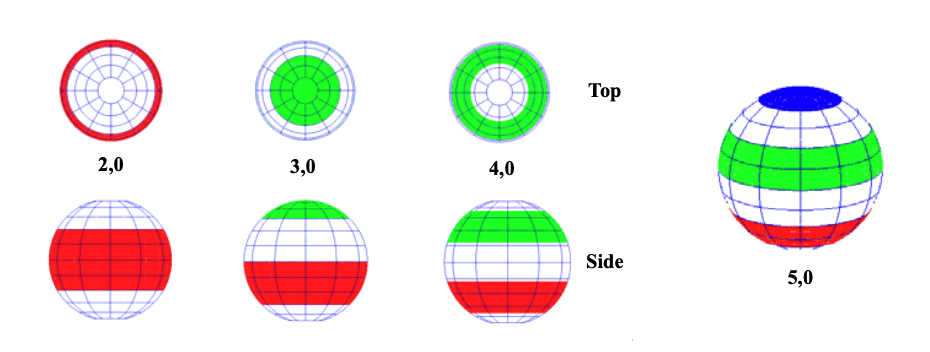
\includegraphics[width=.8\textwidth]{perturbation/zonal}
    \caption{\textbf{Zonal Harmonics.} The band reflects the Earth's oblateness, the shading region indicates regions of additional mass and the numbers link regions  between the views.\cite[]{}.}
    \label{fig:zonal}
\end{figure}

\begin{multicols}{2}
\subsubsection{Sectoral Harmonics}
\textbf{Sectoral Harmonics} occur when $l=m$ and represent bands of longitude (shown in \hyperref[fig:sectoral]{Fig. (\ref*{fig:sectoral})}). The associated Legendre functions, $P_{l,l}[\SIN(\phi_{gc_{sat}})]$ only have zeros at the pole, $\phi = \pm90^{\circ}$, therefore, the only changes in sign are due to the trigonometric functions $\COS(m\lambda)$ and $\SIN(m\lambda)$. On the other hand the terms $[\COS(l\lambda)\hspace*{0.1cm}\text{and}\hspace*{0.1cm}\SIN(l\lambda)]$ are zero for $2l$ different values of $\lambda$. Hence the lines along which the functions $[\COS(l\lambda)\hspace*{0.1cm}\text{and}\hspace*{0.1cm}\SIN(l\lambda)]$ times $P_{l,l}[\SIN(\phi_{gc_{sat}})]$ vanish are meridians of longitude. Each sector represents $l$ positive (shaded) and $l$ negative (white) mass concentrations.
\end{multicols}
\begin{figure}[H]
    \centering
    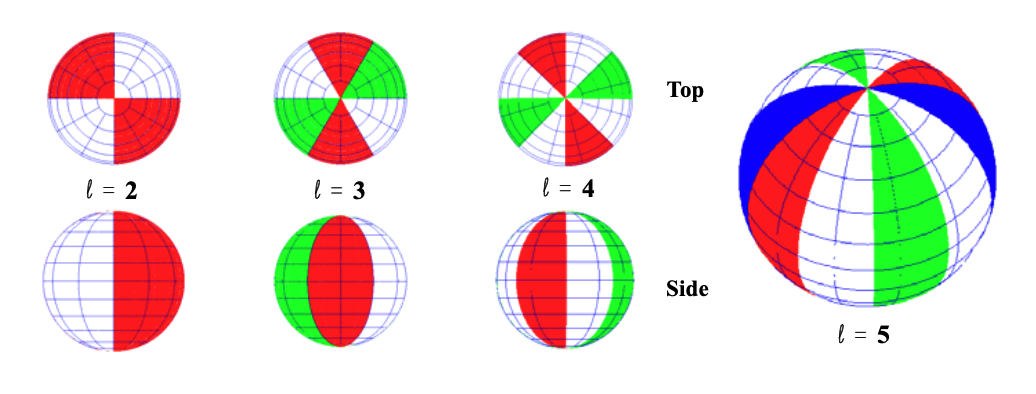
\includegraphics[width=.78\textwidth]{perturbation/sectoral}
    \caption{\textbf{Sectoral Harmonics.} The band reflects the Earth's oblateness, the shading region indicates regions of additional mass and the numbers link regions  between the views.\cite[]{}.}
    \label{fig:sectoral}
\end{figure}

\begin{multicols}{2}
\subsubsection{Tesseral Harmonics}
\textbf{Tesseral harmonics} refer to the cases for $l\neq m\neq0$, the physical depiction is a specific region (tile) of the earth, for the sphere is divided up to a checkerboard array (shown in \hyperref[fig:tesseral]{Fig. (\ref*{fig:tesseral})}). The number of circles of latitude along which $P_{l,m}[\SIN(\phi_{gc_{sat}})]$ is zero is equal to $(l-m)$, whereas the terms $[\COS(l\lambda)\hspace*{0.1cm}\text{and}\hspace*{0.1cm}\SIN(l\lambda)]$ vanish along $2m$ meridians of longitude. These zero lines represent the centre of the latitude/longitude bands.
\end{multicols}

\begin{figure}[hbt]
    \centering
    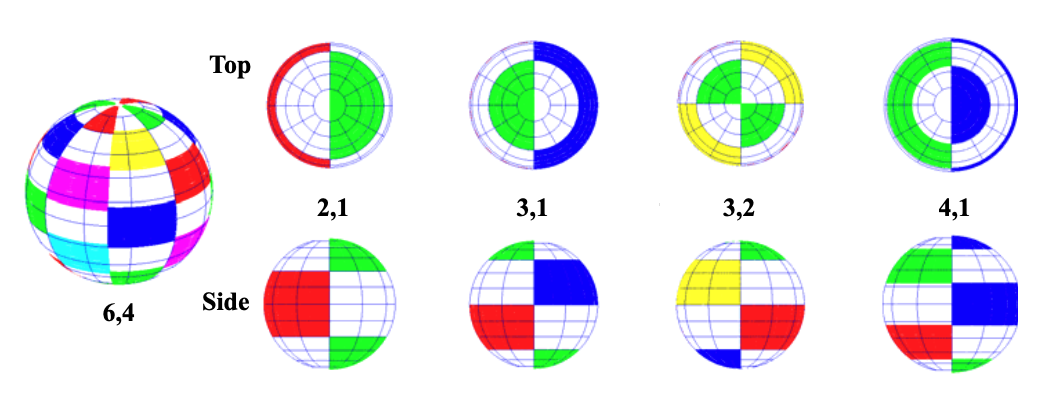
\includegraphics[width=.85\textwidth]{perturbation/tesseral}
    \caption{\textbf{Tesseral Harmonics.} The band reflects the Earth's oblateness, the shading region indicates regions of additional mass and the numbers link regions  between the views.\cite[]{}.}
    \label{fig:tesseral}
\end{figure}


\begin{multicols}{2}
\subsection{Acceleration From Gravitational Potential}
Since we've developed our gravitational potential that describes the uneven distribution of mass for Earth, we then proceed to take the gradient (partial derivative) of the potential and obtain the acceleration term and apply it during orbit propagation. Using matrix differentiation with $\vec{r} = r_I\hat{I} + r_J\hat{J} + r_K\hat{K}$ in the ITRF\footnote{Note that accelerations are usually calculated in body-fixed frame (ECEF, or ITRF), whereas numerical integration are done in an inertial frame (ECI, or GCRF)} frame, we can directly determine the partial derivative of the aspherical potential function. Legendre functions are often differentiated in spherical coordinate, therefore, chain rule is required to find acceleration in cartesian coordinate, as shown below.
\begin{gather}
    \vec{\mathbf{a}} = \frac{\partial U}{\partial r}\Bigg(\frac{\partial r}{\partial \vec{\mathbf{r}}}\Bigg)^T + \frac{\partial U}{\partial\phi_{gc_{sat}}}\Bigg(\frac{\partial\phi_{gc_{sat}}}{\partial\vec{\mathbf{r}}}\Bigg)^T + \frac{\partial u}{\partial\lambda_{sat}}\Bigg(\frac{\partial\lambda_{sat}}{\partial\vec{\mathbf{r}}}\Bigg)^T
\end{gather}
The derivatives of the position vector also proceed directly. Notice that the three partial derivatives below are unit vectors.
\begin{gather}
    \begin{split}
        \frac{\partial r}{\partial\vec{\mathbf{r}}} &= \frac{\vec{\mathbf{r}}^T}{r}\\[0.2cm]
        \frac{\partial\phi_{gc_{sat}}}{\partial\vec{\mathbf{r}}} &= \frac{1}{\sqrt{r_I^2 + r_J^2}}\Big(-\frac{\vec{\mathbf{r}}^{T}r_K}{r^2}+\frac{\partial r_K}{\partial\vec{\mathbf{r}}}\Big)\\[0.2cm]
        \frac{\partial\lambda_{sat}}{\partial\vec{\mathbf{r}}} &= \frac{1}{r_I^2+r_J^2}\Big(r_I\frac{\partial r_J}{\partial\vec{\mathbf{r}}}-r_J\frac{\partial r_I}{\partial\vec{\mathbf{r}}}\Big)
    \end{split}
\end{gather}
Then using the nonspherical portion of \hyperref[eq:final_potential]{Eq. (\ref*{eq:final_potential})}, we can calculate the respective partial derivatives we need for our acceleration
\end{multicols}

\begin{gather}
    \begin{split}
        \frac{\partial U}{\partial r} &= -\frac{\mu}{r}\sum_{l=2}^{\infty}\sum_{m=0}^{l}(\frac{R_{\oplus}}{r})^l(l+1)P_{l,m}[\SIN(\phi_{gc_{sat}})]\Biggl\{C_{l,m}\COS(m\lambda_{sat})+S_{l,m}\SIN(m\lambda_{sat})\Biggr\}\\[0.2cm]
        \frac{\partial U}{\partial\phi_{gc_{sat}}} &= \frac{\mu}{r}\sum_{l=2}^{\infty}\sum_{m=0}^{l}(\frac{R_\oplus}{r})^l\Big\{P_{l,m+1}[\SIN(\phi_{gc_{sat}})]-m\TAN(\phi_{gc_{sat}})P_{l,m}[\SIN(\phi_{gc_{sat}})]\Big\}\Biggl\{C_{l,m}\COS(m\lambda_{sat})+S_{l,m}\SIN(m\lambda_{sat})\Biggr\}\\[0.2cm]
        \frac{\partial U}{\partial\lambda_{sat}} &= \frac{\mu}{r}\sum_{l=2}^{\infty}\sum_{m=0}^{l}(\frac{R_\oplus}{r})^lP_{l,m}[\SIN(\phi_{gc_{sat}})]\Bigg\{S_{l,m}\COS(m\lambda_{sat})-C_{l,m}\SIN(m\lambda_{sat})\Bigg\}
    \end{split}
\end{gather}
\center{\Big\Downarrow}

\begin{gather}
    \begin{split}
        a_I &= \Bigg\{\frac{1}{r}\frac{\partial U}{\partial r}-\frac{r_K}{r^2\sqrt{r_I^2+r_J^2}}\frac{\partial U}{\partial\phi_{gc_{sat}}}\Bigg\}r_I - \Bigg\{\frac{1}{r_I^2+r_J^2}\frac{\partial U}{\partial\lambda_{sat}}\Bigg\}r_J - \frac{\mu r}{r^3}\\[0.2cm]
        a_J &= \Bigg\{\frac{1}{r}\frac{\partial U}{\partial r}-\frac{r_K}{r^2\sqrt{r_I^2+r_J^2}}\frac{\partial U}{\partial\phi_{gc_{sat}}}\Bigg\}r_J + \Bigg\{\frac{1}{r_I^2+r_J^2}\frac{\partial U}{\partial\lambda_{sat}}\Bigg\}r_I - \frac{\mu r}{r^3}\\[0.2cm]
        a_K &= \frac{1}{r}\frac{\partial U}{\partial r}r_K  + \frac{\sqrt{r_I^2+r_J^2}}{r^2}\frac{\partial U}{\partial\phi_{gc_{sat}}}- \frac{\mu r}{r^3}
    \end{split}
\end{gather}
\vspace{0.2cm}
\hrule
\vspace{0.1cm}
\hrule